\documentclass{beamer}

\newcommand{\irptitle}{Remaining Anonymous when using the Bitcoin Protocol}
\usepackage[style=ieee]{biblatex}
\addbibresource{i-d.bib}
\addbibresource{report.bib}
\addbibresource{rfc.bib}

\newcommand\irptopic{Bitcoin}
\newcommand\irpauthor{Thomas A. Grainger}

\newcommand\MYhyperrefoptions{bookmarks=true,bookmarksnumbered=true,
pdfpagemode={UseOutlines},plainpages=false,pdfpagelabels=true,
hidelinks,
pdftitle={\irptitle},%<!CHANGE!
pdfsubject={\irptopic},%<!CHANGE!
pdfauthor={Thomas A. Grainger},%<!CHANGE!
pdfkeywords={Bitcoin, Anonymity, Cryptography, crypto-currencies, Peer to Peer}}
\renewcommand{\biblabelsep}{2em}
\renewcommand{\bibitemsep}{0.2ex}
\renewcommand*{\bibfont}{\tiny}

\usetheme{Madrid} % My favorite!
%\usetheme{Boadilla} % Pretty neat, soft color.
%\usetheme{default}
%\usetheme{Warsaw}
%\usetheme{Bergen} % This template has nagivation on the left
%\usetheme{Frankfurt} % Similar to the default 
%with an extra region at the top.
%\usecolortheme{seahorse} % Simple and clean template
%\usetheme{Darmstadt} % not so good
% Uncomment the following line if you want %
% page numbers and using Warsaw theme%
% \setbeamertemplate{footline}[page number]
%\setbeamercovered{transparent}
\setbeamercovered{invisible}
% To remove the navigation symbols from 
% the bottom of slides%
\setbeamertemplate{navigation symbols}{} 
%
\usepackage{graphicx}
%\usepackage{bm}         % For typesetting bold math (not \mathbold)
%\logo{\includegraphics[height=0.6cm]{yourlogo.eps}}
%
\title[\irptopic]{\irptitle}
\author{\irpauthor}
\institute[U of S]
{
University of Southampton \\
\medskip
{\emph{t.grainger@ecs.soton.ac.uk}}
}
\date{\today}
% \today will show current date. 
% Alternatively, you can specify a date.
%
\begin{document}
%
\begin{frame}
\titlepage
\end{frame}
%
\begin{frame}
\frametitle{Introduction}
\begin{figure}[h!]
    \centering
    \includegraphics[width=0.8\columnwidth]{img/dyn/price}
    \caption{A chart showing the price of Bitcoin over time in USD (source \href{http://bitcoincharts.com/}{bitcoin charts})}
    \label{fig:blockchain}
\end{figure}
\end{frame}
%TODO: TABLE OF CONTENTS?
\begin{frame}
\frametitle{Existing Systems}
\begin{description}
    \item[Central Banking Authorities]\hfill \\
        SEPA and PayPal~\cite{paypal}.
    \item[Unique Token]\hfill \\
        NetCash~\cite{netcash}.
    \item[Blind-signing]\hfill \\
        Chaumian e-Cash\cite{chaum}.
    \item[Digital Signature Chain]\hfill \\
        B-Money\cite{b-money}.
\end{description}
\end{frame}
%

\begin{frame}
\frametitle{Existing Systems}
\framesubtitle{B-Money}

\begin{figure}[h!]
    \centering
    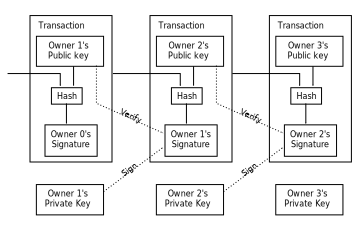
\includegraphics[width=0.8\columnwidth]{img/Bitcoin_Transaction_Visual}
    \caption{A chain of digital signatures representing value transfer.
    (source \protect\cite{satoshi})}
    \label{fig:chain-spend}
\end{figure}
\end{frame}

\begin{frame}
\frametitle{The Bitcoin Protocol}
The Bitcoin block chain is a concrete implementation of B-Money\\
But it uses a block chain.
\begin{block}
{Blocks\ldots}
\begin{itemize}
\item contain the latest transactions
\item refer to the previous block in the chain by hash value
\item must meet a ``proof-of-work'' requirement
\end{itemize}
\end{block}
\end{frame}

\begin{frame}
\frametitle{The Bitcoin Protocol}
\framesubtitle{The block chain}
\begin{figure}[h!]
    \centering
    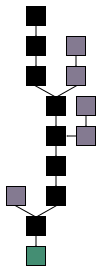
\includegraphics[angle=-90,width=0.8\columnwidth]{img/Blockchain}
    \caption{A diagram showing invalid blocks (grey) being invalidated by a block chain with greater totally difficulty (black). (based on work from \href{http://theymos.com/}{theymos})}
    \label{fig:blockchain}
\end{figure}
\end{frame}

\begin{frame}
\frametitle{The Bitcoin Protocol}
\framesubtitle{Hash Power}
\begin{figure}[h!]
    \centering
    \includegraphics[width=0.8\columnwidth]{img/dyn/speed-lin-ever.png}
    \caption{A chart showing the total hash power of the Bitcoin network (source \href{http://bitcoin.sipa.be/speed-lin-ever.png}{SIPA})}
    \label{fig:blockchain}
\end{figure}
\end{frame}

\begin{frame}
\frametitle{De-Anonymization Techniques}
\begin{description}

\item[Multi-Input Transactions] If a user cannot fulfill the value of a transaction by spending a  single previous output, the client will combine multiple inputs\cite{reid-anon}.
\item[Change Addresses] Because each output must be redeemed in it's entirety transactions of values smaller than the smallest output available to a wallet, the Bitcoin client uses ``change addresses'' so as to retain the remaining value.

\end{description}
\end{frame}

\begin{frame}
\frametitle{De-Anonymization Techniques}
\begin{figure}[h!]
    \centering
    \includegraphics[width=0.8\columnwidth]{img/group_addresses}
    \caption{Two users send money to $k_{SR}$. Under the Multi-Input  heuristic $k_{a1}, k_{a2} and k_{a3}$ and $k_{b1}, k_{b2}$ are contracted into  some user $a$ and some user $b$. Under the change address heuristic  $k_{a4}$ and $k_{b3}$ are also contracted into user $a$ and user $b$  respectively. }
    \label{fig:blockchain}
\end{figure}
\end{frame}



\begin{frame}
\frametitle{References}
\footnotesize{
\printbibliography
}
\end{frame}
 
\begin{frame}
\centerline{The End}
\end{frame}
% End of slides
\end{document} 